% Drawing 154/06-16 -- folder 154, batch 06, archive page 118 (PDF page 119).
% Transcription: en haut à gauche, un dessin en couleur de la bande supersingulière (droites vert clair, ligne médiane en tirets rouges et bleus, droites rouges en losanges, arcs rouges en haut et en bas) ; en haut à droite, deux arcs vert clair en forme d'arche, aux sommets marqués, sous la légende « \struck{\ill{}} $\alpha \geqslant 2$ sommets verts clairs » ; ailleurs, des croquis au crayon : des droites $D$, $D'$, $D''$ qui se coupent, les points $a$, $a'$, $x$, $x'$ et les étiquettes $\omega_D$, $\omega_{D'}$, $\omega_{D''}$, un repère fléché
% Kind: supersingular band; two arches with marked vertices; pencil sketches of lines D, D', D''. Method 2 (schematic redraw from the facsimile). Status: partial.
% Notes: Top left, a colour drawing of the supersingular band (light green lines, middle line in red and blue dashes, red lines in lozenges, red arcs at the top and the bottom). Top right, two light green arches with marked vertices, under the legend « alpha >= 2 sommets verts clairs » (a struck word before it). Elsewhere pencil sketches: lines D, D', D'' that cut one another, the points a, a', x, x', and the labels omega_D, omega_D', omega_D'', an arrowed frame; these are drawn only in part (the frame, two lines with a, a', and the main labels); the pencilled formulas are text of the transcription. Read from the page view.
% Coordinates: 1 unit = 1 mm = 1/100 of the crop width (bbox in page fractions: [0.202, 0.073, 0.927, 0.47]).
% Redrawn by Claude (claude-opus-5-5), issue #73, 2026-11-07; not checked by a human; not compiled (no TeX in the session).
% Rights: reproduces part of the work -- behind RENDER_TRANSCRIPTS, never published by itself.
\documentclass[tikz,border=3pt]{standalone}
\usepackage{amsmath,amssymb}
\usetikzlibrary{patterns,arrows.meta}
\tikzset{Or/.style={orange!90!black}, Ye/.style={yellow!80!orange}, Lg/.style={green!60!black!70}, Dg/.style={green!45!black}, Br/.style={brown!80!black}, Rd/.style={red!85!black}, Bl/.style={blue!70!black}, Gy/.style={black!40}, pencil/.style={black!45}, struck/.style={black!35}, mark/.style={circle,draw,inner sep=1.3pt}, pt/.style={circle,fill,inner sep=0.9pt}, opt/.style={circle,draw,fill=white,inner sep=1.1pt}}
\begin{document}
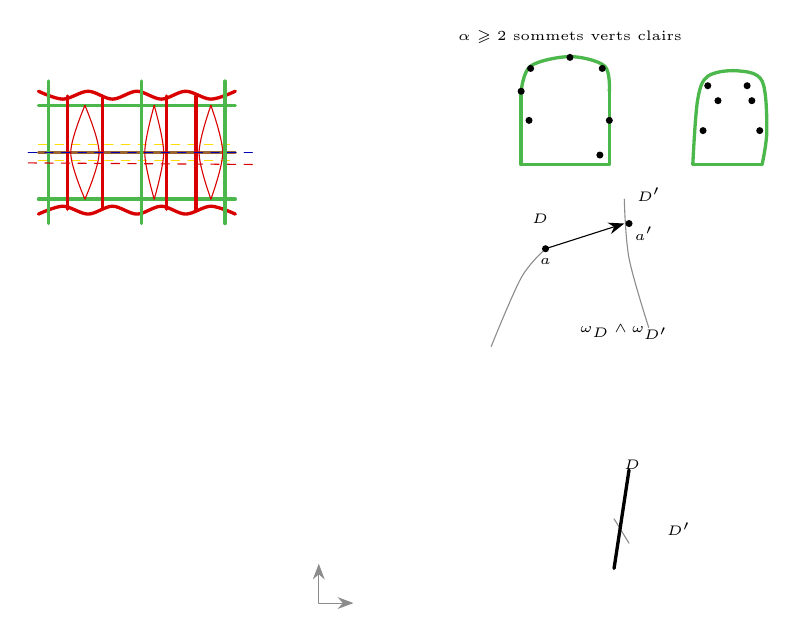
\begin{tikzpicture}[x=1mm,y=1mm,line cap=round,line join=round,font=\scriptsize]
\draw[Lg,very thick] (2.5,-10.6) -- (27.5,-10.6);
\draw[Lg,very thick] (2.5,-22.5) -- (27.5,-22.5);
\draw[Br,very thick] (2.5,-16.6) -- (27.5,-16.6);
\draw[Ye,dashed] (2.5,-15.6) -- (27.5,-15.6);
\draw[Ye,dashed] (2.5,-17.6) -- (27.5,-17.6);
\draw[Rd,very thick] plot[smooth, tension=0.55] coordinates {(2.5,-8.8) (5.6,-9.8) (8.8,-8.8) (11.9,-9.8) (15,-8.8) (18.1,-9.8) (21.2,-8.8) (24.4,-9.8) (27.5,-8.8)};
\draw[Rd,very thick] plot[smooth, tension=0.55] coordinates {(2.5,-24.4) (5.6,-23.4) (8.8,-24.4) (11.9,-23.4) (15,-24.4) (18.1,-23.4) (21.2,-24.4) (24.4,-23.4) (27.5,-24.4)};
\draw[Rd,very thick] (6.2,-9.4) -- (6.2,-23.8);
\draw[Rd,very thick] (10.6,-9.4) -- (10.6,-23.8);
\draw[Rd,very thick] (15.6,-9.4) -- (15.6,-23.8);
\draw[Rd,very thick] (18.8,-9.4) -- (18.8,-23.8);
\draw[Rd,very thick] (22.5,-9.4) -- (22.5,-23.8);
\draw[Rd,very thick] (26.2,-9.4) -- (26.2,-23.8);
\draw[Rd] plot[smooth, tension=0.55] coordinates {(8.4,-10.6) (6.6,-16.6) (8.4,-22.5)};
\draw[Rd] plot[smooth, tension=0.55] coordinates {(8.4,-10.6) (10.2,-16.6) (8.4,-22.5)};
\draw[Rd] plot[smooth, tension=0.55] coordinates {(17.2,-10.6) (16,-16.6) (17.2,-22.5)};
\draw[Rd] plot[smooth, tension=0.55] coordinates {(17.2,-10.6) (18.4,-16.6) (17.2,-22.5)};
\draw[Rd] plot[smooth, tension=0.55] coordinates {(24.4,-10.6) (22.9,-16.6) (24.4,-22.5)};
\draw[Rd] plot[smooth, tension=0.55] coordinates {(24.4,-10.6) (25.9,-16.6) (24.4,-22.5)};
\draw[Lg,very thick] (3.8,-7.5) -- (3.8,-25.6);
\draw[Lg,very thick] (15.6,-7.5) -- (15.6,-25.6);
\draw[Lg,very thick] (26.2,-7.5) -- (26.2,-25.6);
\draw[Bl,dashed] (1.2,-16.6) -- (30,-16.6);
\draw[Rd,dashed] (1.2,-17.9) -- (30,-18.1);
\draw[Lg,very thick] (63.8,-18.1) -- (63.8,-8.8);
\draw[Lg,very thick] plot[smooth, tension=0.55] coordinates {(63.8,-8.8) (65,-5.6) (70,-4.4) (74.4,-5.6) (75,-8.8)};
\draw[Lg,very thick] (75,-8.8) -- (75,-18.1);
\draw[Lg,very thick] (63.8,-18.1) -- (75,-18.1);
\node[pt] at (63.8,-8.8) {};
\node[pt] at (65,-5.9) {};
\node[pt] at (70,-4.5) {};
\node[pt] at (74.1,-5.9) {};
\node[pt] at (75,-12.5) {};
\node[pt] at (64.8,-12.5) {};
\node[pt] at (73.8,-16.9) {};
\node[inner sep=1pt] at (70,-1.9) {\tiny $\alpha\geqslant2$ sommets verts clairs};
\draw[Lg,very thick] plot[smooth, tension=0.55] coordinates {(85.6,-18.1) (86.2,-10) (87.5,-6.9) (91.2,-6.2) (94.4,-7.5) (95,-13.8) (94.4,-18.1)};
\draw[Lg,very thick] (85.6,-18.1) -- (94.4,-18.1);
\node[pt] at (87.5,-8.1) {};
\node[pt] at (92.5,-8.1) {};
\node[pt] at (86.9,-13.8) {};
\node[pt] at (94.1,-13.8) {};
\node[pt] at (88.8,-10) {};
\node[pt] at (93.1,-10) {};
\draw[pencil] plot[smooth, tension=0.55] coordinates {(60,-41.2) (63.8,-32.5) (66.9,-28.8)};
\draw[-{Stealth[length=2mm]}] (66.9,-28.8) -- (76.9,-25.6);
\draw[pencil] plot[smooth, tension=0.55] coordinates {(76.9,-22.5) (77.5,-30) (80,-38.8)};
\node[pt] at (66.9,-28.8) {};
\node[pt] at (77.5,-25.6) {};
\node[inner sep=1pt] at (66.9,-30.4) {\tiny $a$};
\node[inner sep=1pt] at (79.4,-26.9) {\tiny $a'$};
\node[inner sep=1pt] at (66.2,-25) {\tiny $D$};
\node[inner sep=1pt] at (80,-21.9) {\tiny $D'$};
\node[inner sep=1pt] at (76.9,-39.4) {\tiny $\omega_D\wedge\omega_{D'}$};
\draw[-{Stealth[length=2mm]},pencil] (38.1,-73.8) -- (42.5,-73.8);
\draw[-{Stealth[length=2mm]},pencil] (38.1,-73.8) -- (38.1,-68.8);
\draw[pencil] (77.5,-66.2) -- (75.6,-63.1);
\draw[very thick] (75.6,-69.4) -- (77.5,-56.9);
\node[inner sep=1pt] at (77.9,-56.2) {\tiny $D$};
\node[inner sep=1pt] at (83.8,-64.4) {\tiny $D'$};
\end{tikzpicture}
\end{document}
